\chapter{Appendix}

\section{Risk Analysis}
It is important to account for any risks that may happen during the development of this architecture. By establishing a contingency plan for common risks, hindrances within the development process will be minimized. The following risks can seen in Figure 12.1 below.

\begin{figure}[h]
	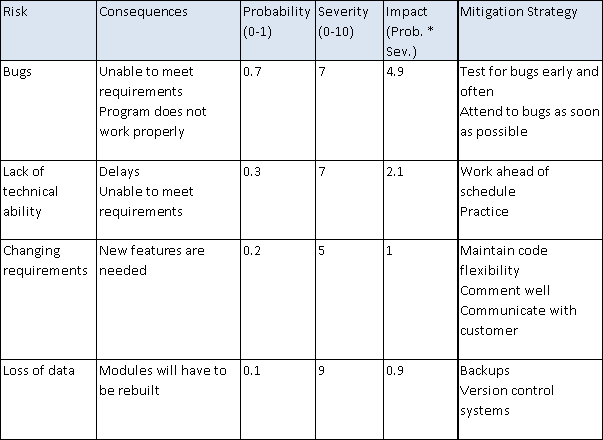
\includegraphics[width=\linewidth]{images/risk_analysis.png}
	\caption{Risk Table}
	\label{fig:risk table}
	\centering
\end{figure}

\clearpage
\newpage

\section{Development Timeline}
The development timeline shows a clear view of each team member’s responsibilities and roles in this project. Each team member’s progress can be traced across the time periods shown below in Figure 12.2.

\begin{figure}[h]
	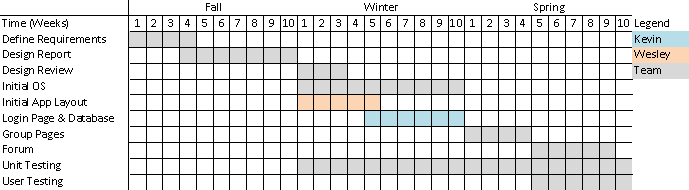
\includegraphics[width=\linewidth]{images/timeline.png}
	\caption{Development Timeline}
	\label{fig:timeline}
	\centering
\end{figure}